\newpage % Rozdziały zaczynamy od nowej strony.
\section{Eksperymenty}
\subsection{Zbiór  danych}
Dane są kluczową częścią głębokiego uczenia. Duży zbiór danych oznaczonych adnotacjami na poziomie pikseli jest potrzebny do wytrenowania wydajnego modelu segmentacji semantycznej. Typowe zestawy danych do segmentacji semantycznej to Cityscapes, PASCAL VOC i ADE20K. Podobnie w przypadku klasyfikacji sceny wymagany jest duży zbiór danych z odpowiednią informacją o etykiecie. Popularne zestawy danych do klasyfikacji scen obejmują  NYUv2, SUN RGB-D, Matterport3D i ScanNet.



Zbiór danych powinien ściśle odpowiadać założeniom postawionym w pracy. Inferencja wymaga użycia kamery Kinect. Zatem zbiór danych powinien zawierać kategorie scen, segmentacje obrazów oraz najlepiej być ujętym przez kamerę Kinect wersji pierwszej.

Po prześledzeniu wielu zbiorów danych udało się sprostać powyższym wymaganiom, uzyskując dwa podobne zbiory danych - \texttt{NYUv2} oraz \texttt{SUN RGBD}. Ostatecznie wybrano \texttt{NYUv2} z uwagi, że zbiór ten został zawiera zdjecia
pomieszczeń, w które nie są posprzątane. Fakt ten uznano, za ważny, iż uważano, że będzie przekładał się na lepsze rezultaty w naturalnych warunkach. Co więcej \texttt{NYUv2} jest też chętniej cytowany niż \texttt{SUN RGBD} (rys. \ref{fig:sun-vs-nyu}).

\begin{figure}[ht!]
    \centering
    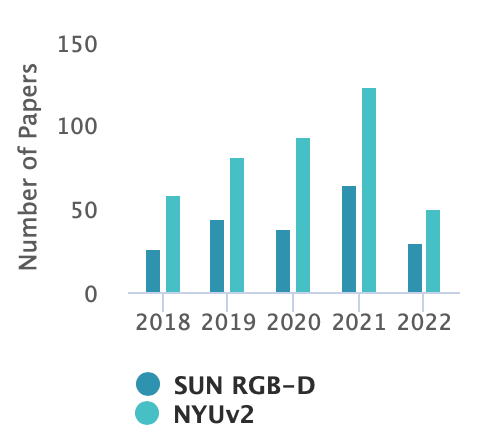
\includegraphics[width=0.5\textwidth]{img/stats-dataset.png}
    \caption[]{Szacowana liczba cytowań w latach 2018-2022 \href{https://paperswithcode.com/dataset/sun-rgb-d}{[paperswithcode.com]}}
    \label{fig:sun-vs-nyu}
\end{figure}

\subsection{Analiza zbioru danych}
Eksploracyjna analiza danych (ang. EDA) to proces eksploracji i zrozumienia cech zbioru danych przed zbudowaniem modelu. Omówione zostanie znaczenie EDA w głębokim uczeniu oraz możliwości wykorzystania do poprawy wydajności i interpretowalności modeli głębokiego uczenia.

Jakość danych

Jednym z głównych powodów, dla których EDA jest ważne w wizji komputerowej, jest to, że może pomóc w identyfikacji problemów ze zbiorem danych, takich jak brakujące wartości, wartości odstające lub nieprawidłowe etykiety, które mogą wpłynąć na wydajność modelu wizji komputerowej. Przeprowadzając EDA, możemy uzyskać głębsze zrozumienie danych i zidentyfikować wszelkie problemy, które należy rozwiązać przed zbudowaniem modelu.

Wstępne przetwarzanie danych

EDA może być również wykorzystana do określenia, które kroki przetwarzania wstępnego (ang. preprocessing), takie jak augmentacja, są niezbędne do poprawy wydajności modelu wizji komputerowej. Badając dane i rozumiejąc ich charakterystykę, jesteśmy w stanie lepiej dostosować różne techniki wstępnego przetwarzania danych.

Identyfikacja tendencyjności

EDA może być również wykorzystana do identyfikacji potencjalnych błędów w zbiorze danych, takich jak skośne rozkłady klas, które mogą wpływać na wydajność modelu widzenia komputerowego i prowadzić do niesprawiedliwych prognoz. Przeprowadzając EDA, możemy zidentyfikować wszelkie uprzedzenia w danych i podjąć kroki w celu ich rozwiązania przed zbudowaniem modelu.

% Wnioski

% Podsumowując, prowadzenie EDA jest ważne w wizji komputerowej, ponieważ może pomóc poprawić wydajność modelu, zwiększyć jego interpretowalność i zapewnić, że model jest sprawiedliwy i bezstronny. EDA może być wykorzystana do identyfikacji problemów ze zbiorem danych, wyboru odpowiednich cech, wstępnego przetwarzania danych, zrozumienia zachowania modelu i zidentyfikowania potencjalnych stronniczości. Przeprowadzając EDA, możemy uzyskać głębsze zrozumienie danych oraz poprawić wydajność i interpretowalność modelu widzenia komputerowego.

EDA przeprowadzone na zbiorze NYUv2 dostarczyło wielu interesujących szczegółów. W zbiorze domyślnie znajduje się 795 przykładów trenujących oraz 654 przykładów testujących. Ze zbioru testowego wyodrębniono zbiór walidacyjny stanowiący 20\% zbioru testowego. Ponadto sprawdzono rozkład klas na przesztrzeni całego zbioru danych.
W przypadku zadania segmentacji semantycznej do dyspozycji był wybór 894, 40 lub 13 klas przedmiotów. Im rozróżnialność była większa tym większe okazywały się dysproporcje w rozkładzie. Histogramy dla 13 i 40 klas przedstawiono na rysunku \ref{fig:rozklad-segm}.
Podobna sytuacja miała miejsce dla zadania klasyfikacji z tą różnicą, iż scalania klas należało dokonać ręcznie. Taki krok był kluczowy, gdyż pierwotny rozkład był silnie zdominowany przez kilka klas.
Ostatecznie wybrano 13 klas dla klasyfikacji (rys. \ref{fig:7 klas dystrybucja}) oraz scalone 7 dla segmentacji (rys. \ref{fig:7 klas dystrybucja}).
\begin{figure}[ht!]
    \centering
    \begin{subfigure}[b]{0.49\textwidth}
        \centering
        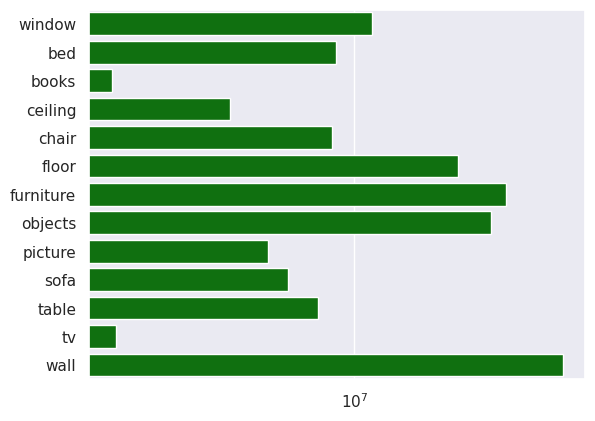
\includegraphics[width=\textwidth]{seg13.png}
        \caption{Rozkład dla 13 klas.}
        \label{fig:rozklad-13klas-seg}
    \end{subfigure}
    \hfill
    \begin{subfigure}[b]{0.49\textwidth}
        \centering
        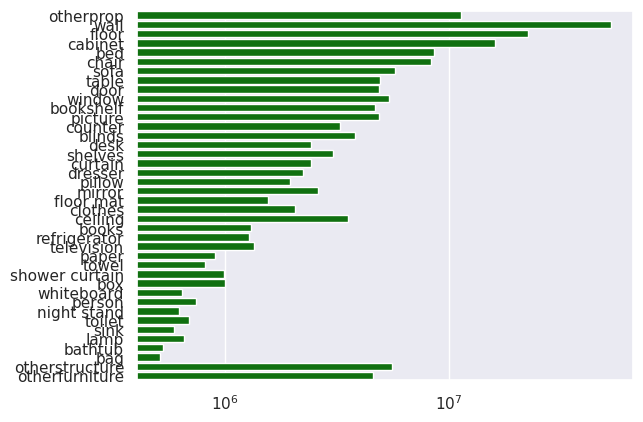
\includegraphics[width=\textwidth]{seg40.png}
        \caption{Rozkład dla 40 klas.}
        \label{fig:rozklad-40klas-seg}
    \end{subfigure}
    \caption[]{Porównanie rozkładu ilości pixeli dla zadania segmentacji semantycznej.}
    \label{fig:rozklad-segm}
\end{figure}
\begin{figure}
    \centering
    \begin{subfigure}[b]{0.49\textwidth}
        \centering
        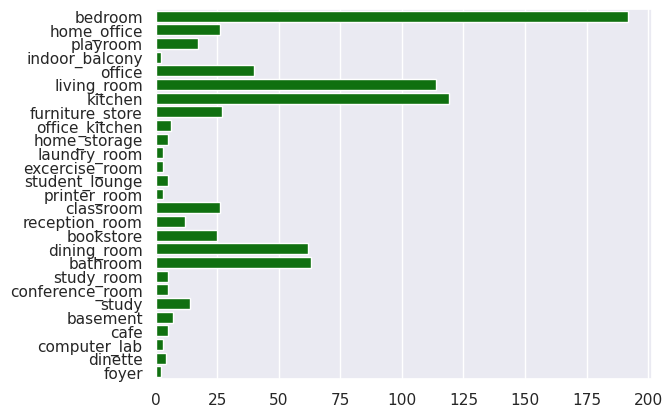
\includegraphics[width=\textwidth]{classification.png}
        \caption{Oryginalny rozkład klas.}
        \label{fig:27 klas dystrybucja}
    \end{subfigure}
    \hfill
    \begin{subfigure}[b]{0.49\textwidth}
        \centering
        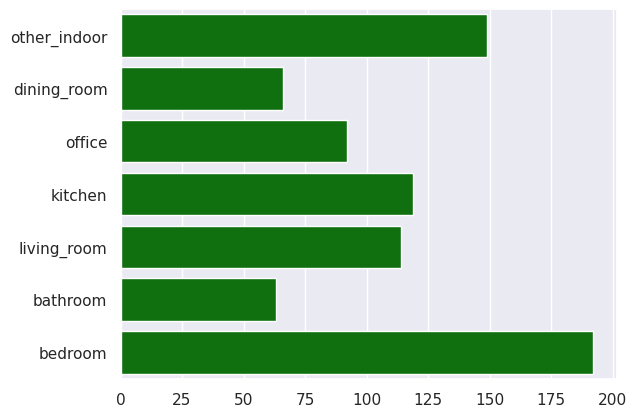
\includegraphics[width=\textwidth]{classification-merged.png}
        \caption{Rozkład klas po scaleniu.}
        \label{fig:7 klas dystrybucja}
    \end{subfigure}
    \caption[]{Porównanie rozkładu klas dla zadania klasyfikacji sceny.}
\end{figure}

% * wykorzystanie TU NICR
% * Wersje segmentacji: 13, 40 i 8xx klasowa
% * ile obrazków w jakich zbiorach.
% * wstawić przykładowe obrazki z datasetu
% * Konkatenacja dla klas dla klasyfikacji - dlaczego?
% * EDA - histogramy klas

\subsection{Opis eksperymentów}
\noindent
Przygotowanie danych

Obrazy RGB zostały poddane normalizacji ze średnią (0.485, 0.456, 0.406) oraz odchyleniem standardowym (0.229, 0.224, 0.225), która odpowiada parametrom rozkładu normlanego na zbiorze ImageNet. Baza ImageNet służyła do wytrenowania enkodera, a więc pierwszej części modelu.

Istnieje kilka różnych technik normalizacji, które mogą być stosowane w problemach z widzeniem komputerowym, takich jak normalizacja min-max i normalizacja rozkładem normalnym.  W pracy ,,Normalization Techniques in Training DNNs:
Methodology, Analysis and Application'' Lei et. al. \cite{huang2020normalization}, autorzy udowadjniają, że normalizacja stabilizuje i przyśpiesza trening oraz prawdopodobnie prowadzi do
do poprawy generalizacji. 

Normalizacja jest ważnym krokiem przetwarzania wstępnego w problemach widzenia komputerowego, ponieważ może pomóc w poprawieniu wydajności modelu. Normalizacja odnosi się do procesu skalowania danych wejściowych tak, aby miały w przybliżeniu średnią 0 i odchylenie standardowe 1. Pomaga to zapewnić, że dane wejściowe są w spójnym zakresie i mają podobny rozkład, co może poprawić model.
\noindent
Model

Jako  model użyto DeepLabv3, który rozszerzono o dodatkową głowę klasyfikacyjną. Umieszczono ją naturalnie zaraz za enkoderem, a przed dekoderem. Głowa klasyfikacyjna przedstawia się jako jako sieć w pełni połączona (FC) z dwiema warstwami.  

TO TRZEBA ZWIUZALIZOWAĆ!
\begin{addmargin}[6mm]{0mm}
    \begin{lstlisting}[
        language=Python,
        numbers=left,
        firstnumber=1,
        caption={Struktura głowy klasyfikacyjnej},
        aboveskip=0pt
    ]
    nn.AdaptiveAvgPool2d((1, 1)),
    nn.Flatten(),
    nn.BatchNorm1d(num_filters),
    nn.Dropout(p=0.25),
    nn.Linear(num_filters, out_features=256, bias=False),
    nn.ReLU(inplace=True),
    nn.BatchNorm1d(256),
    nn.Dropout(p=0.25),
    nn.Linear(in_features=256, out_features=scene_classes, bias=False),
    nn.Softmax(dim=1),
    \end{lstlisting}
    \end{addmargin}

\noindent
Funkcja straty

W obu przypadkach jako funkcję straty wykorzystano ważoną entropię skrośną. Wagi odzwierciedłały odwrotność liczności w zbiorze. Dla klasyfikacji liczona była ilość klas, natomiast dla segmentacji ilość pixeli.

\noindent
Uczenie

Uczenie odbywało się co najwyżej 50 epok aż do ustalenia się straty na zbiorze walidacyjnym. Krok uczenia był zmienny zgodnie z polityką One Cycle (rys.\ref{fig:one-cycle-policy}).


\begin{figure}[ht!]
    \centering
    \begin{subfigure}[b]{0.32\textwidth}
        \centering
        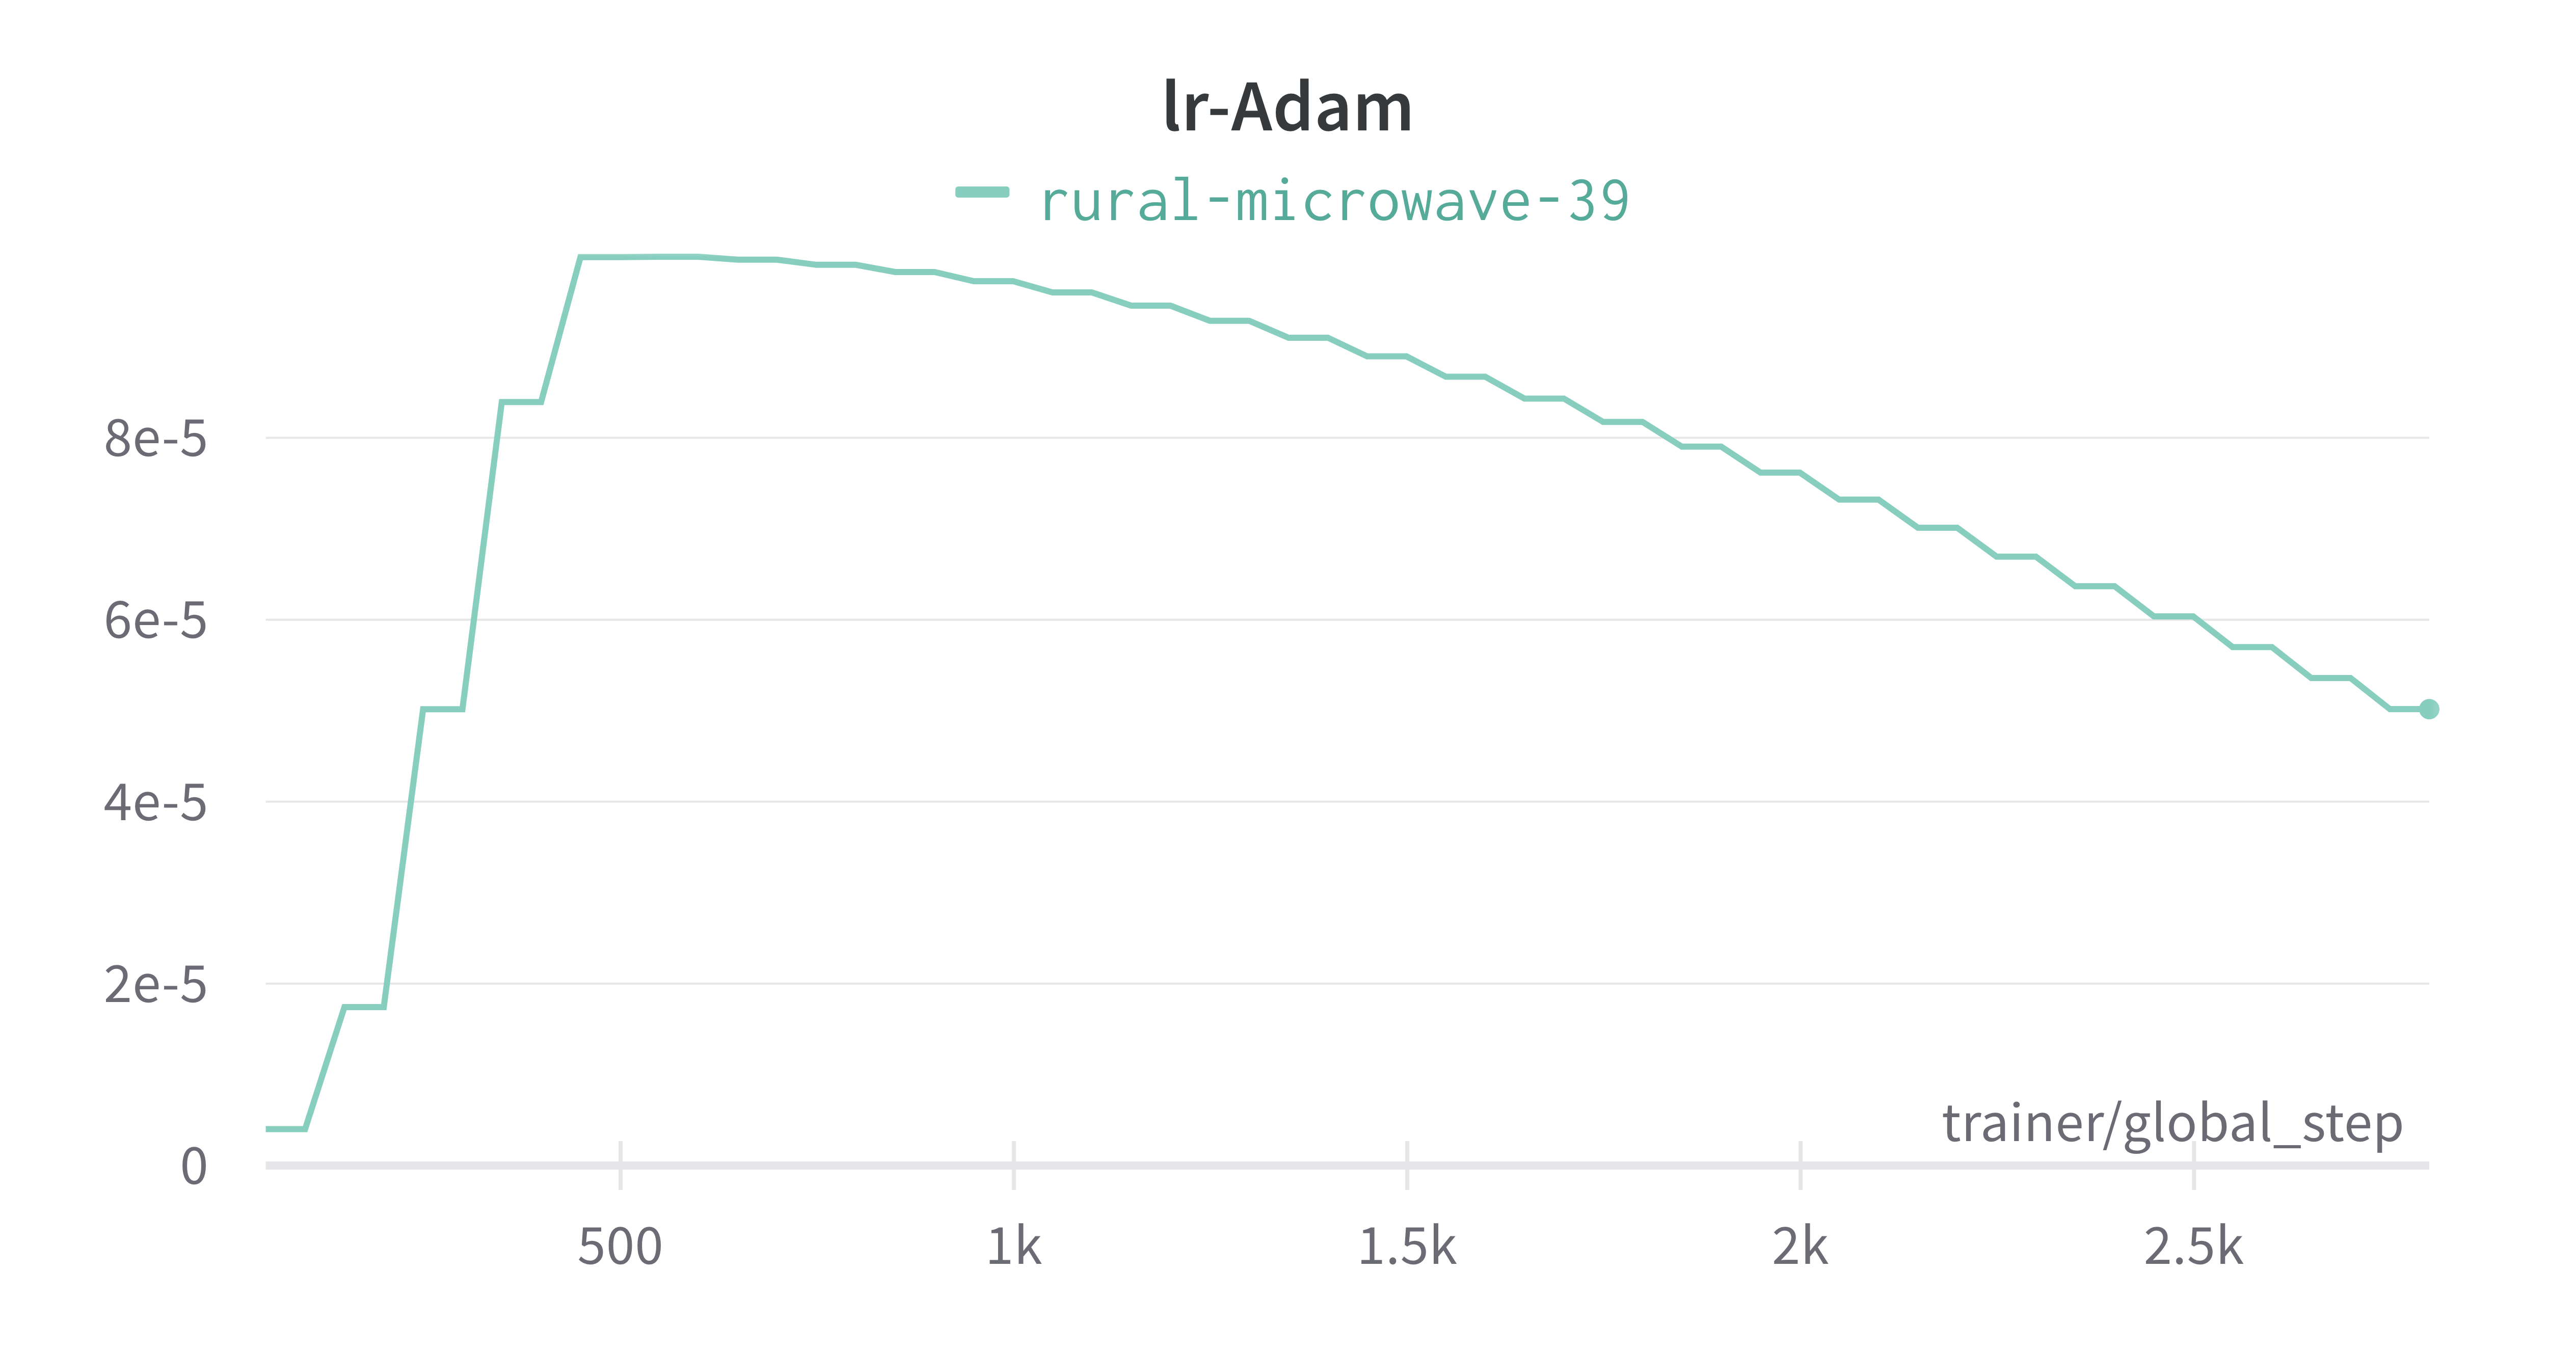
\includegraphics[width=\textwidth]{seg-lr.png}
        \caption{Segmentacja semantyczna.}
        % \label{fig:rozklad-13klas-seg}
    \end{subfigure}
    \hfill
    \begin{subfigure}[b]{0.32\textwidth}
        \centering
        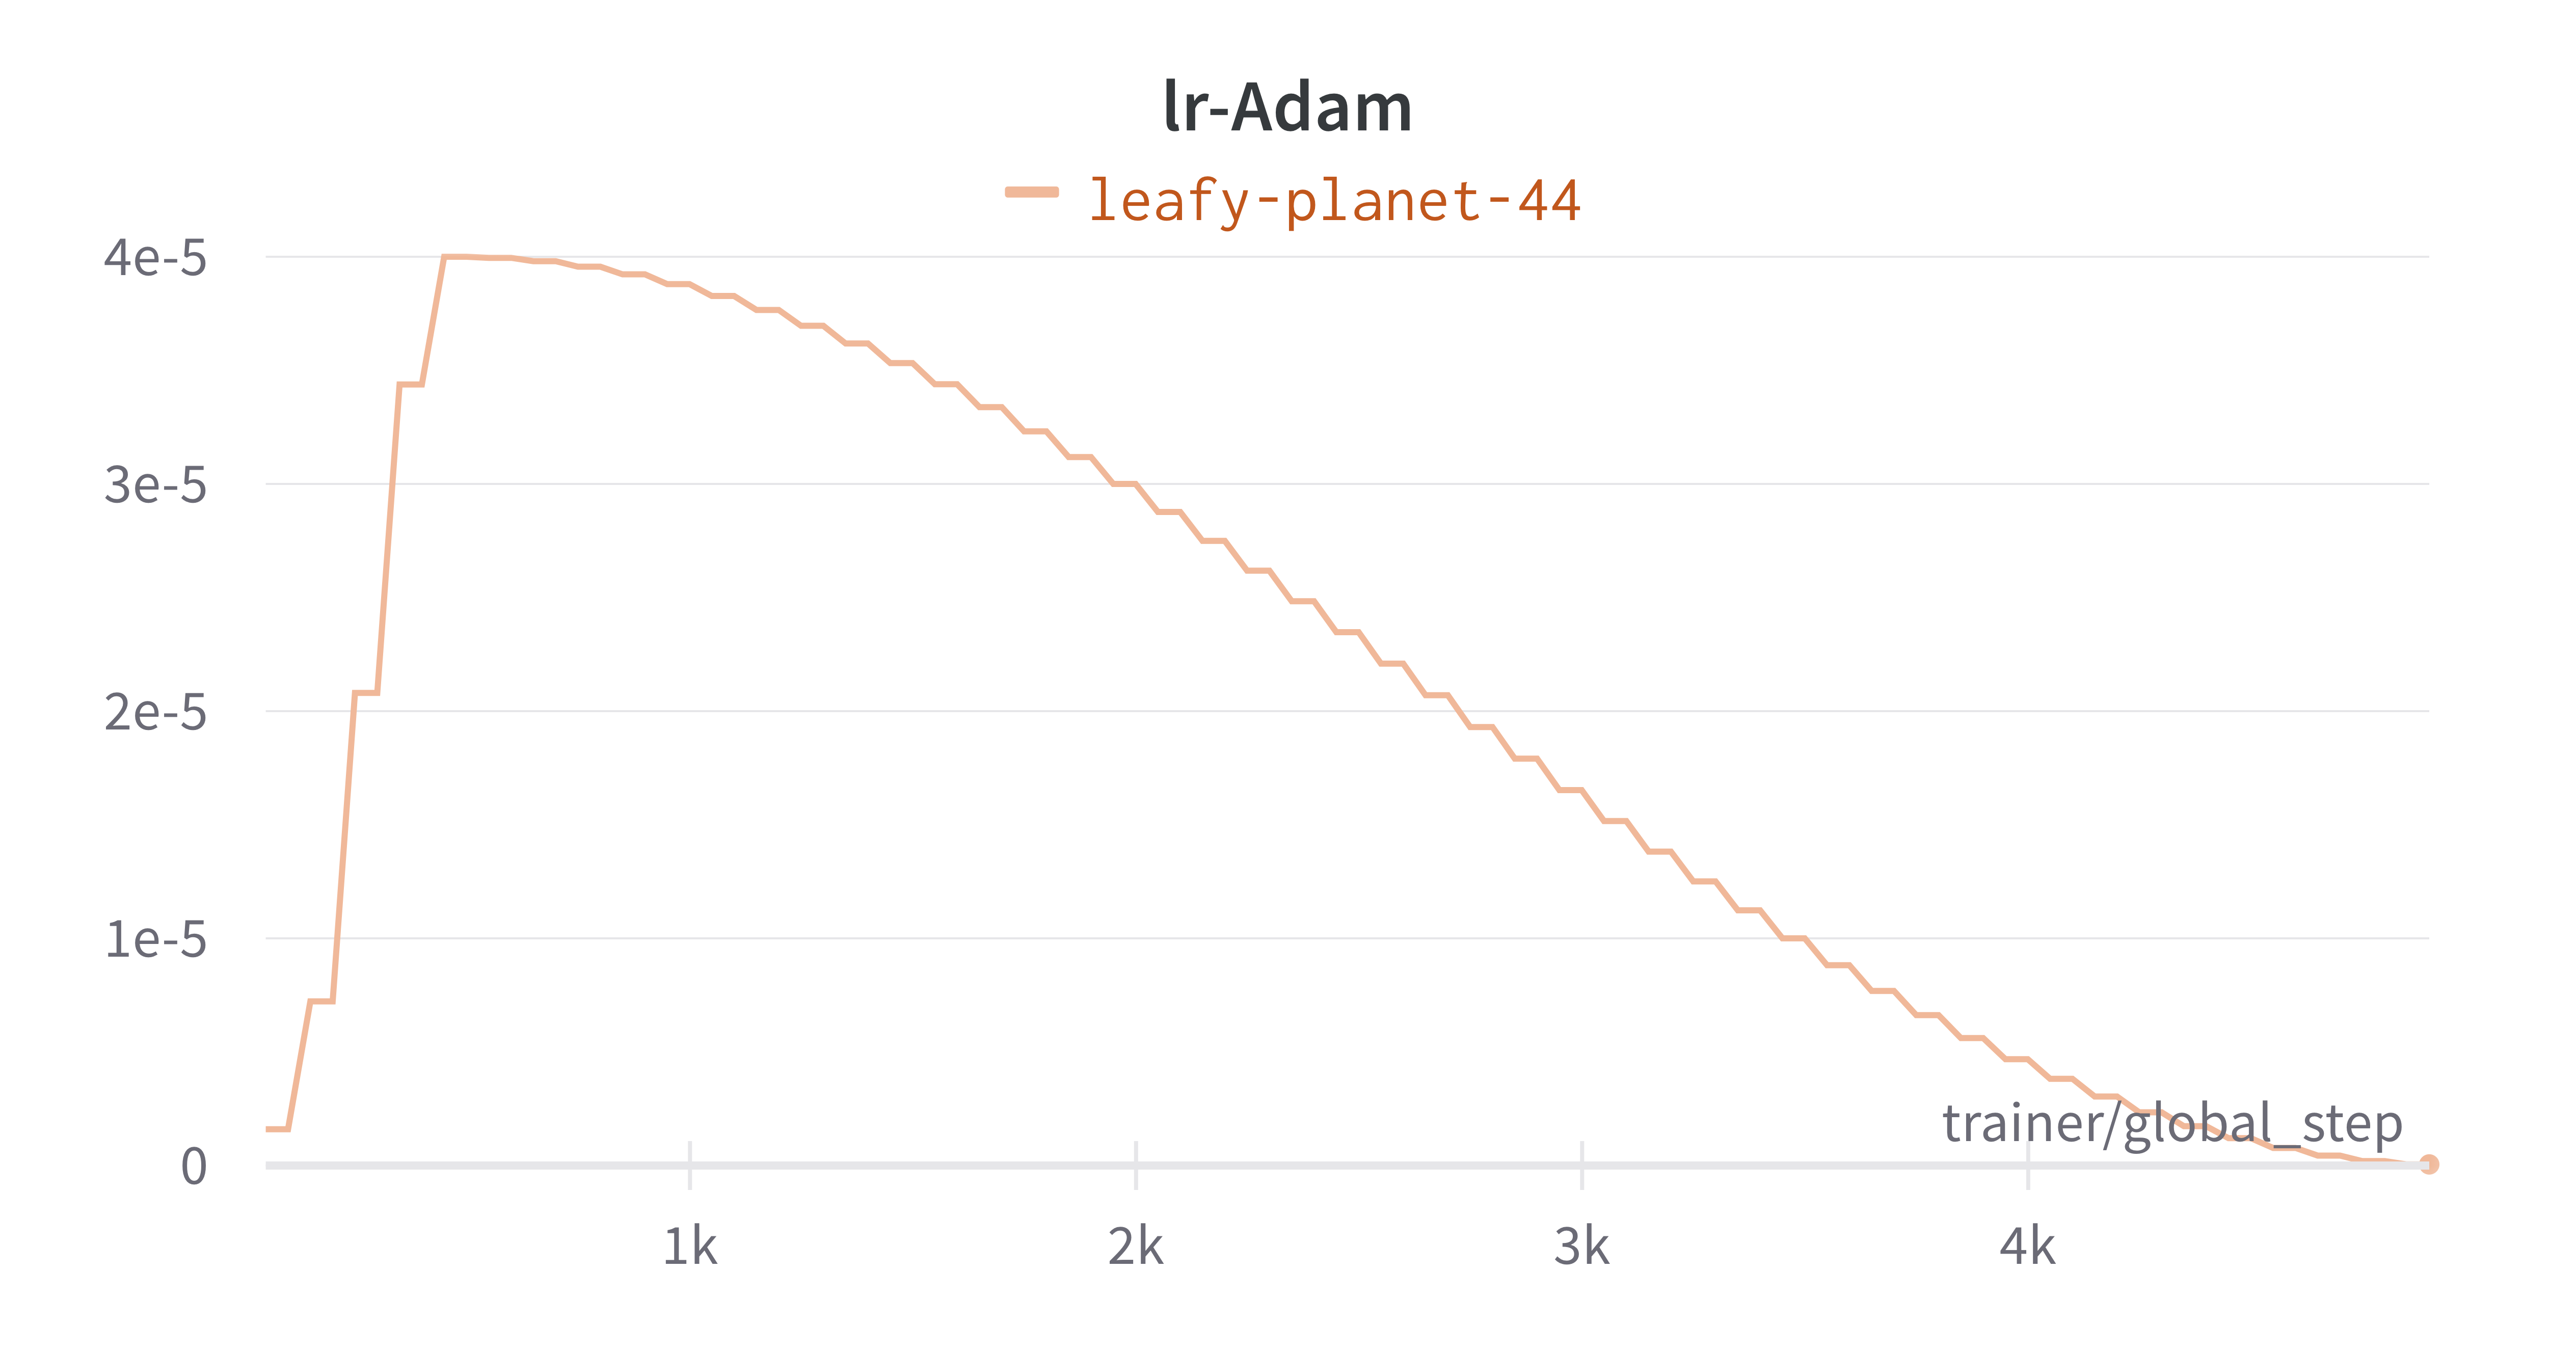
\includegraphics[width=\textwidth]{class-lr.png}
        \caption{Klasyfikacja sceny.}
        % \label{fig:rozklad-40klas-seg}
    \end{subfigure}
    \hfill
    \begin{subfigure}[b]{0.32\textwidth}
        \centering
        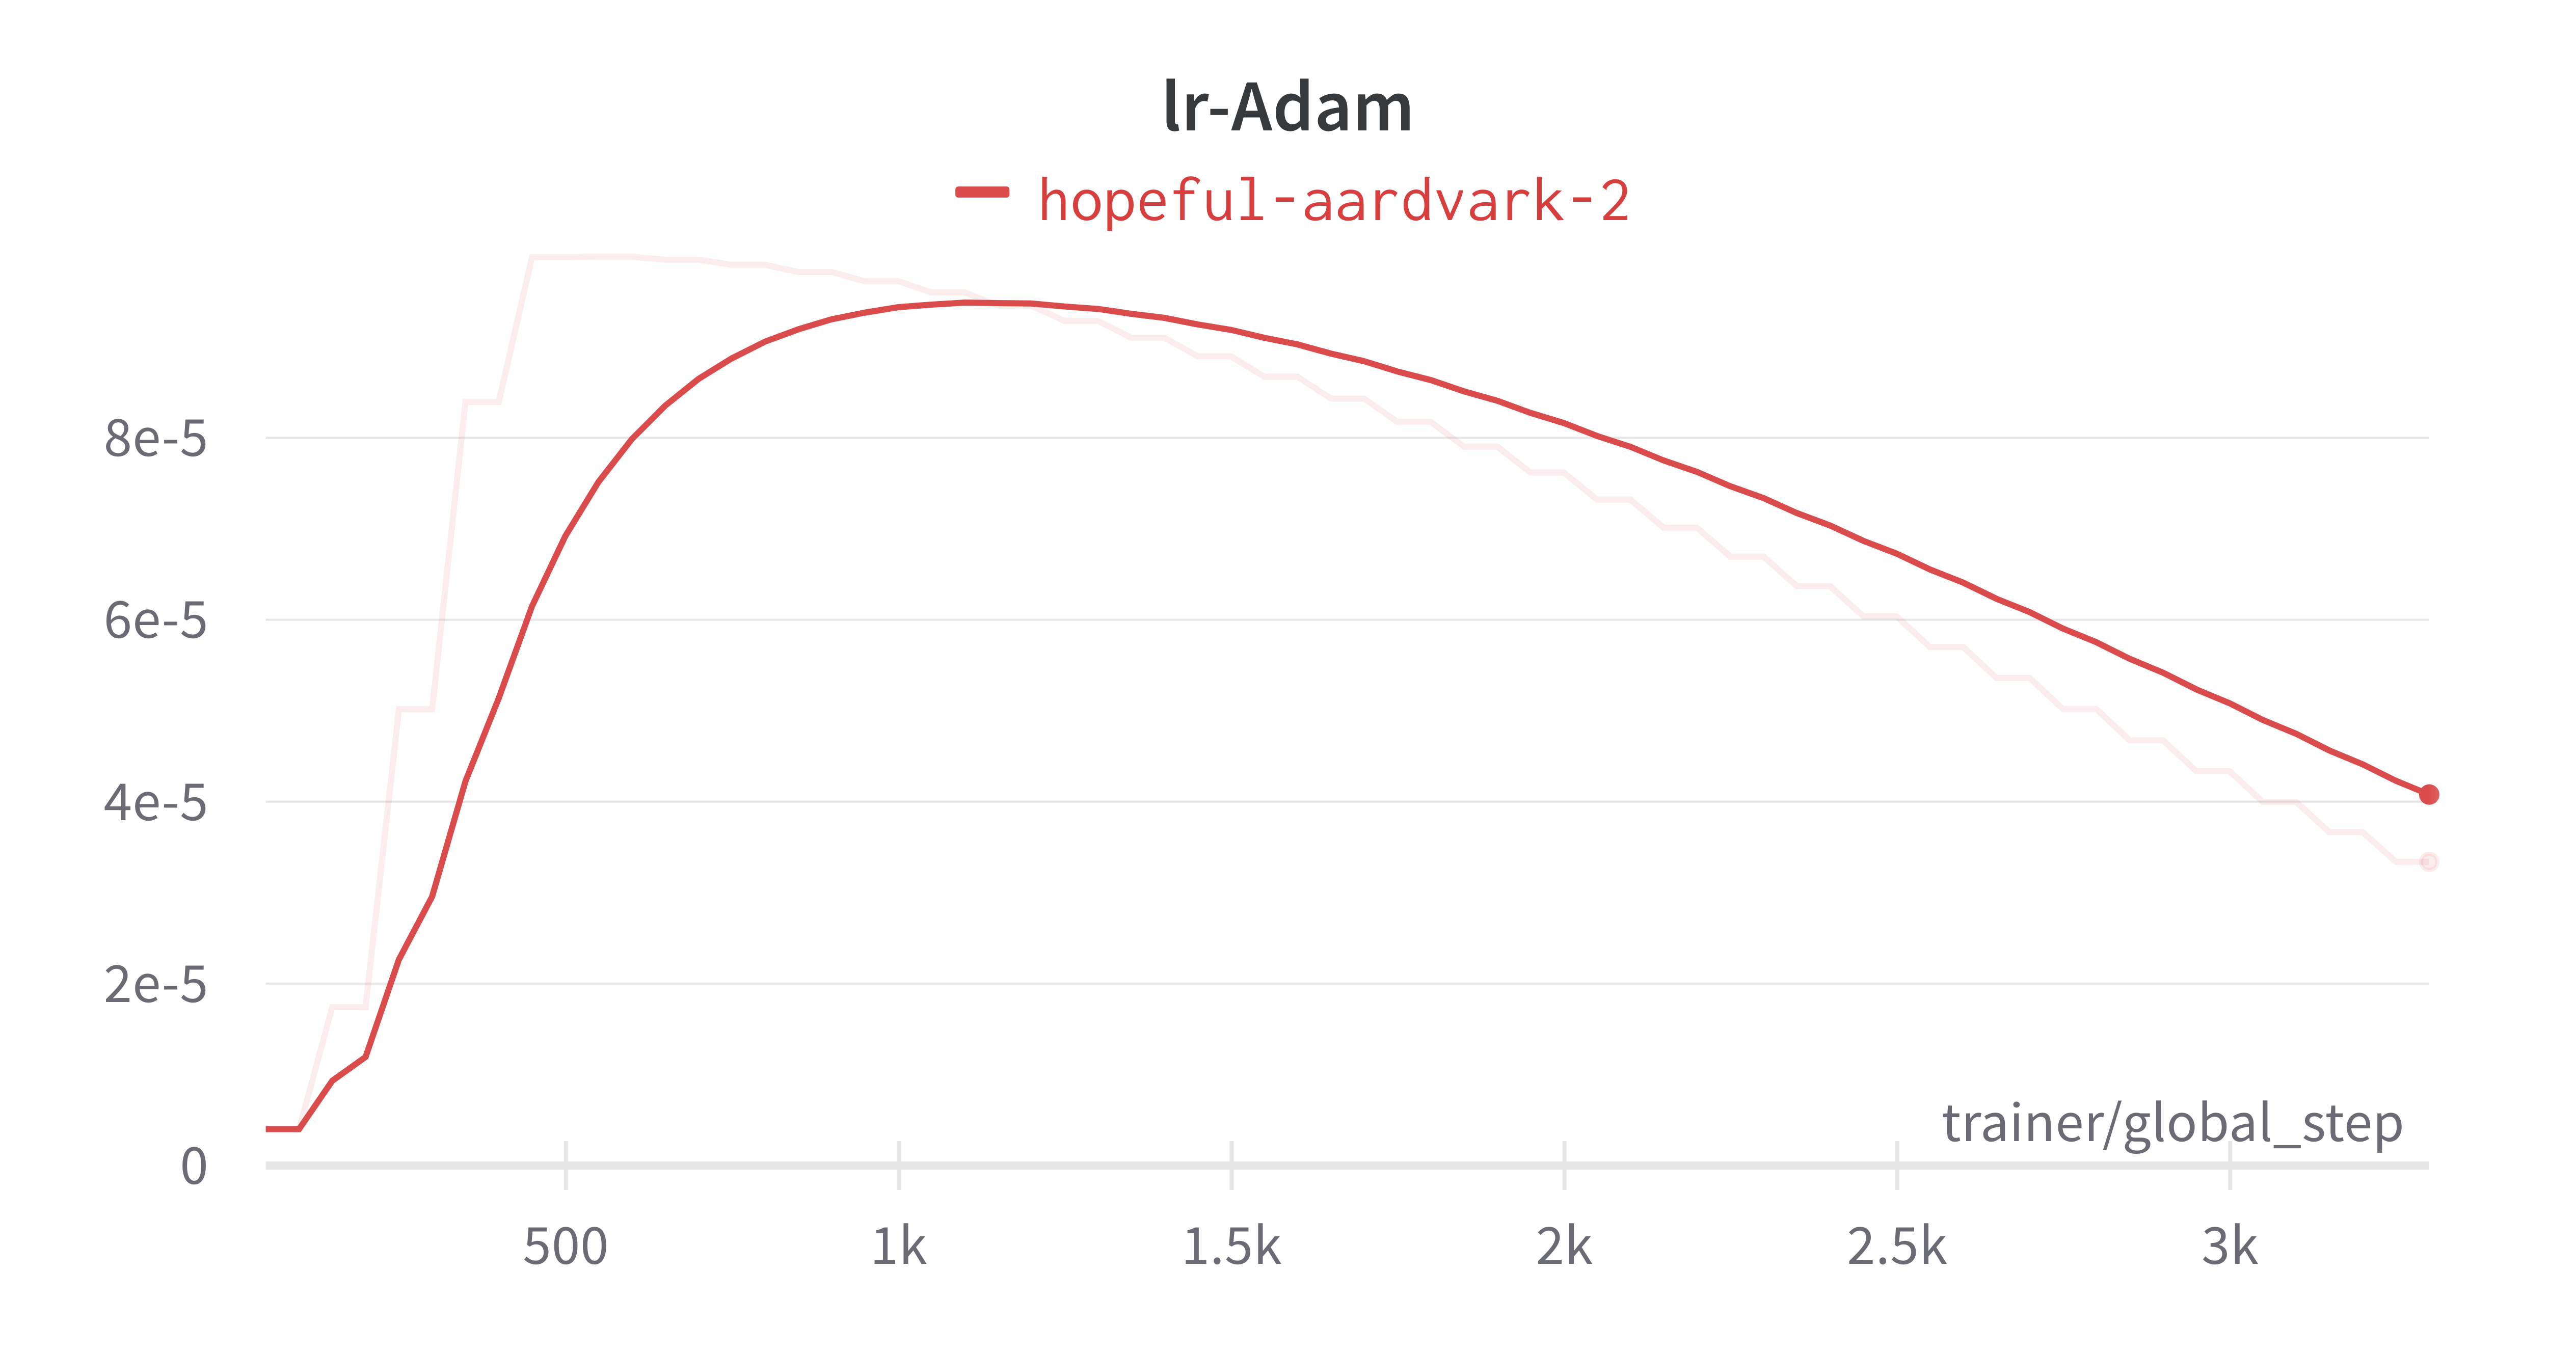
\includegraphics[width=\textwidth]{multitask-lr.png}
        \caption{Uczenie wielozadaniowe.}
        % \label{fig:rozklad-40klas-seg}
    \end{subfigure}
    \caption[]{One cycle learning rate scheduler policy}
    \label{fig:one-cycle-policy}
\end{figure}
\subsection{Wyniki}

\begin{table}[]
    \centering
    \begin{tabular}{c|cc}
        zadanie/{[}\%{]} & Acc jednozadaniowe & Acc wielozadaniowe \\ \hline
        segmentacja      & 67.87               & 67.48  \footnotesize{\textbf{$-$0.39}}        \\
        klasyfikacja     & 65.50               & 67.45  \footnotesize{\textbf{+1.95}}        \\ \hline
    średnia          & 66.69               & 67.47  \footnotesize{\textbf{+0.78}}       
\end{tabular}
\caption{Porównanie dokładności dla uczenia jedno- i wielozadaniowe.}
\label{tab:acc-por}
\end{table}

\begin{figure}[ht!]
    \centering
    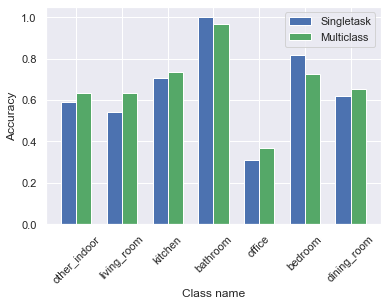
\includegraphics[width=0.75\textwidth]{scene_comp.png}
    \caption{Porównanie dokładności dla każdej z klas w zadaniu klasyfikacji pomieszczeń}
    \label{fig:scene_comp}
\end{figure}

\begin{figure}[ht!]
    \centering
    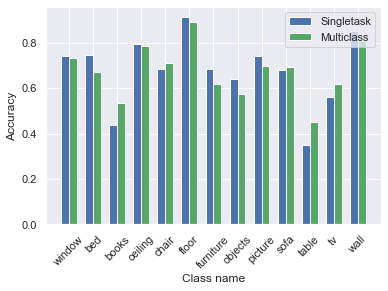
\includegraphics[width=0.75\textwidth]{seg_comp.png}
    \caption{Porównanie dokładności dla każdej z klas w zadaniu segmentacji semantycznej}
    \label{fig:seg_comp}
\end{figure}
Ucznie wielozadaniowe w rozważanym przypadku nieznacznie poprawia wyniki sieci (tab. \ref{tab:acc-por}). Dla zadania segmentacji semantycznej otrzymujemy spadek jakości o 0.39 punkta procentowego. Zadanie klasyfikacji poprawia się o 1.95 p.p. w porównaniu z uczeniem jednozadaniowym. Ostatecznie otrzymujemy zysk na poziomie 0.78 punkta procentego na średniej z zadań. Poprawa jest niewielka, jednak jest to dużu sukces biorąc pod uwagę, że mamy do dyspozycji 2 razy mniej parametrów niz w przypadku dwóch osobnych sieci. Przekłada się to bezpośrednio na czas inferencji, który w przypadku robotyki i systemów czasu rzeczywistego jest kluczowy.

Wartym zobaczenia jest fakt, iż uczenie wielozadaniowe poprawia wyniki dla klas które osiągają najsłabsze rezultaty w uczeniu jednozadaniowym. Poprawie ulega klasa office (rys. \ref{fig:scene_comp}) dla klasyfikacji oraz klasy books oraz table (rys. \ref{fig:seg_comp}) dla segmentacji semantycznej. Powodem jest prawdopodbnie mniejsze obciążenie (bias) modelu spowodowane faktem wzajemnej regularyzacji obu zadań w procesie uczenia. Innymi słowy, model ma mniejszą tendencję do przeuczenia.